\documentclass{article}
\usepackage{graphicx}
\usepackage{wrapfig}

\begin{document}
\title{Factors Affecting Extinction}

\begin{figure}
    
\includegraphics[width=\linewidth]{ITU.jpg}
\end{figure}
\maketitle
\author{Rinalds Lipenitis \and Jakub Mráz \and
Adam Rosenørn \and Costel Gutu \and Richard Kentoš}
\begin{center}
\date{March 2023}
\end{center}

\newpage

\section{Exercise 1}


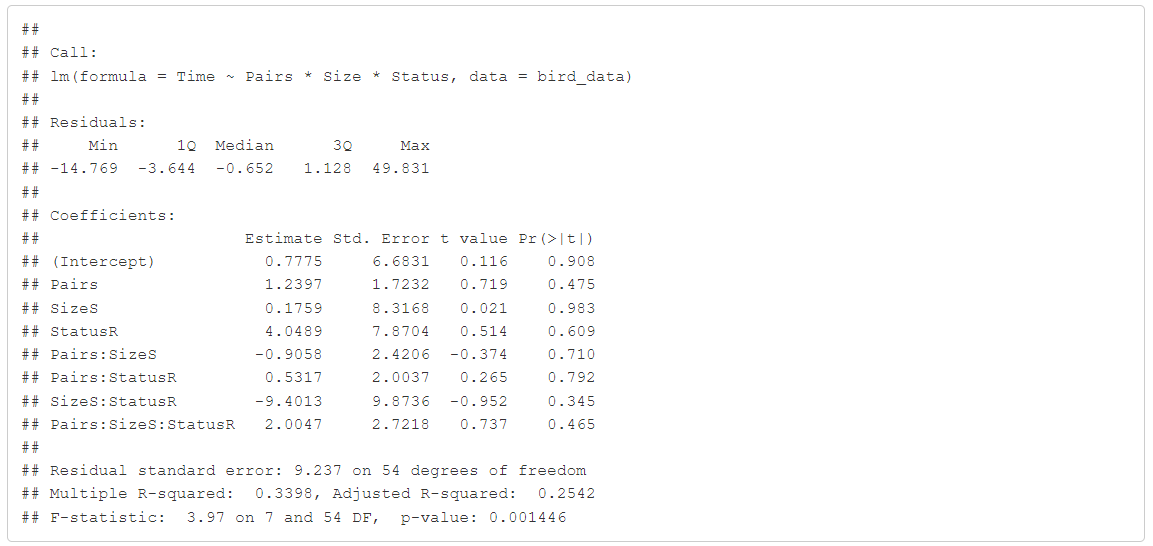
\includegraphics[scale=0.5]{tables/all-multiplied.png}


\begin{center}
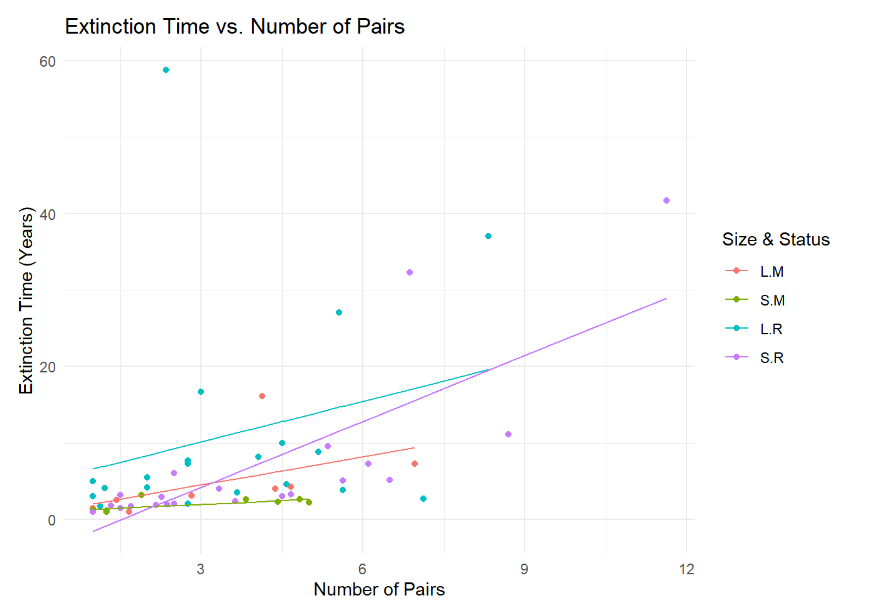
\includegraphics[scale=0.5]{graphs/graph1.png}
\end{center}

\section{Exercise 2}

\begin{center}
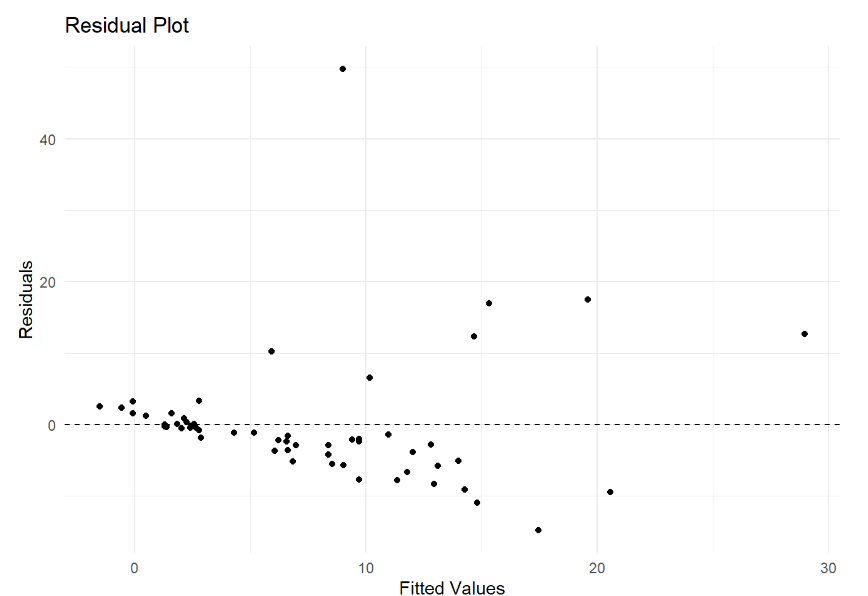
\includegraphics[scale=0.5]{graphs/residual.png}
\end{center}


When examining the residuals, we look for: \\

Homoscedasticity: The residuals should have constant variance across the range of fitted values. If the spread of residuals seems to change across the fitted values, a transformation may be needed.
The variance of the residuals becomes bigger and bigger as the value being fitted (number of pairs + extinction time) goes up. \\

Independence: There should be no patterns or trends in the residuals. If you notice any patterns or trends, it might indicate that a variable is missing from the model, or a transformation is needed.
There appears to be a slight downward slope pattern. \\

Outliers: Look for points that stand out from the rest, as they may be outliers. Investigate these points further to determine if they are errors or if they represent genuine observations. You may consider removing outliers if they are affecting the model’s performance. \\
Biggest outlier: \\
Species: Raven \\
Time: 58.82 \\
Pairs: 2.35 \\
Size: L \\
Status: R \\

Normality: Ideally, the residuals should be approximately normally distributed. If the residuals exhibit a non-normal distribution, you may need to consider a transformation of the dependent variable or use a different modeling approach.

\begin{center}
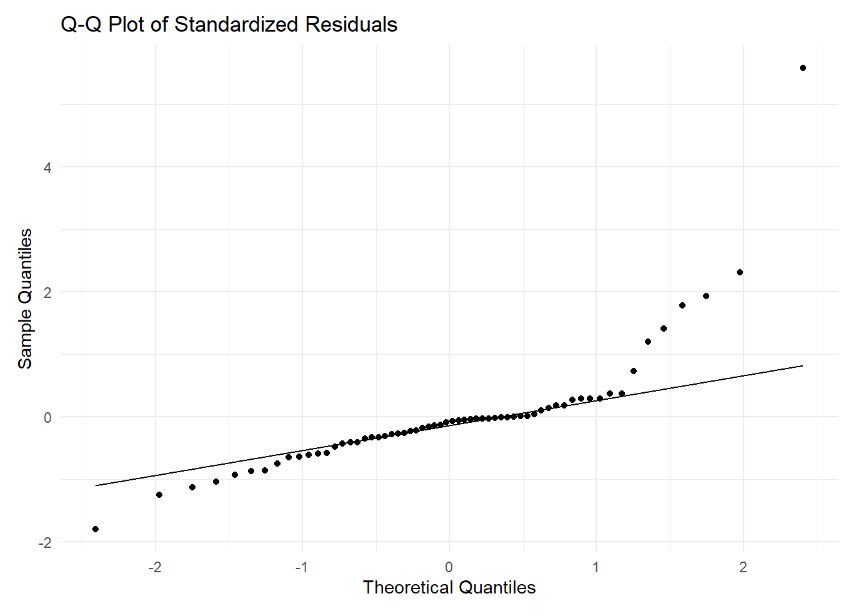
\includegraphics[scale=0.5]{graphs/qq-residuals.png}
\end{center}

The residuals appear to be normally distributed except for the lower and upper ends, where they become more skewed, this suggests that a data transformation may be necessarry.


\section{Exercise 3}

\begin{center}
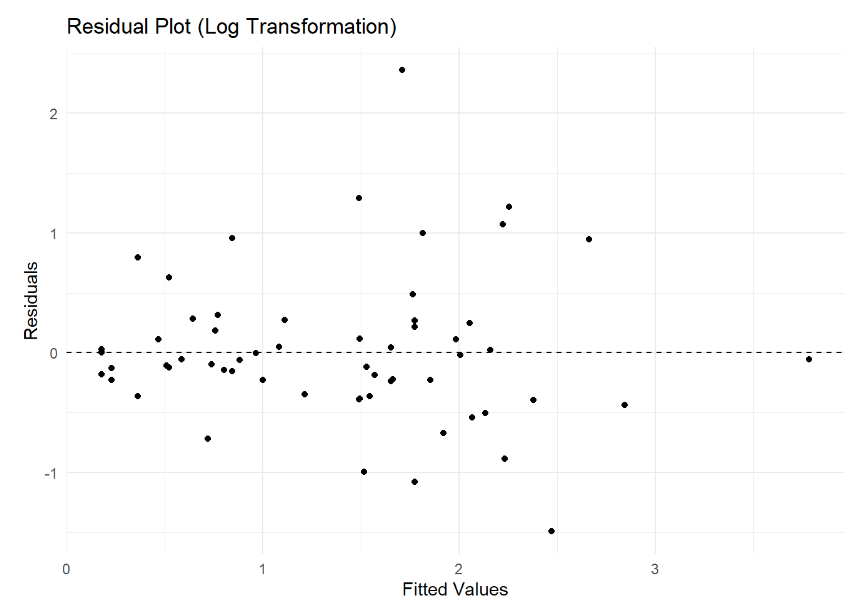
\includegraphics[scale=0.5]{graphs/graph-log.png}
\end{center}

\begin{center}
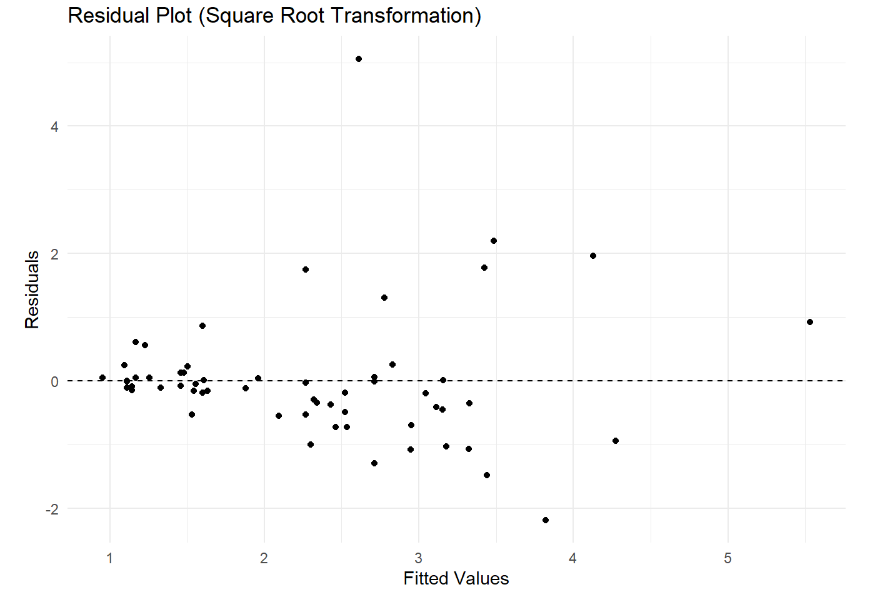
\includegraphics[scale=0.5]{graphs/graph-sqrt.png}
\end{center}

\begin{center}
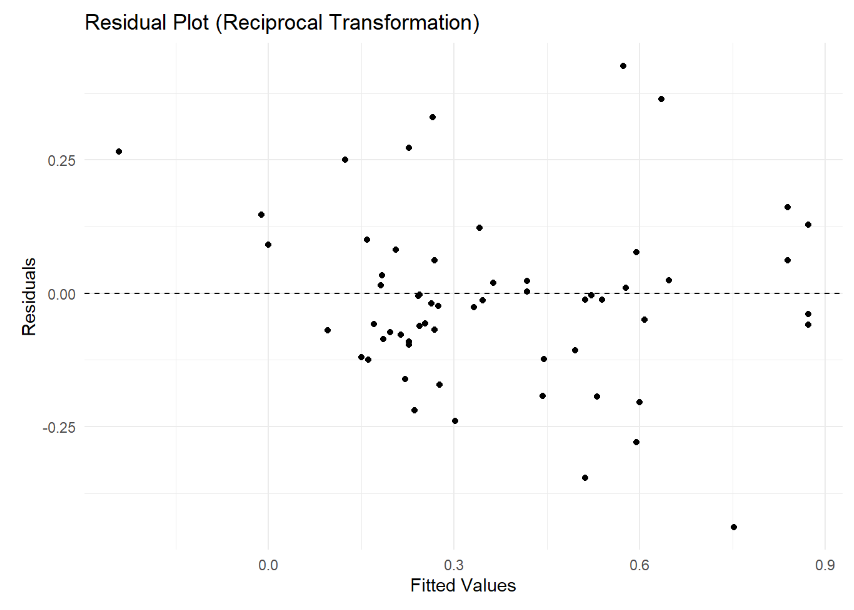
\includegraphics[scale=0.5]{graphs/graph-over.png}
\end{center}

Immediately, we can tell that the square transformation does not improve the model. To compare the log and reciprocal transformation, we will use Q-Q plots again.

Based on the Q-Q plots, the log transformation seems to be the best fit for the majority of the fitted data points.

\section{Exercise 4}
Results can be significantly impacted by the outlier in each end of the scale. Outliers can also affect the measures of the central tendency, more specifically mean, median and mode. Moreover, they can also affect standard deviation and range - the spread of the data.

We believe that is is vital for us to keep the outliers in the dataset for various reasons:

1. Outliers provide important information about the data distribution. To be more specific, they can indicate the presence of extreme or unusual values, which might be beneficial for understanding the range and variability of our data. For instance,  the outlier for the Peregrine species in this dataset indicates that it has a much lower average time until it becomes extinct than the other species. This could also be because of the specific environmental or ecological factors.

2. Preventing loss of information and biased analysis. Outliers may be representing rare but important occurrences that we should not leave out. Removing them might result in a distorted view of the true data distribution and lead to incorrect conclusions. For instance, if we decided to remove the outlier for the Raven species in this dataset, we would miss the fact that it has much longer average extinction time than the other species.

3. Allowing more robust statistical analysis. Methods such as robust regression or non-parametric tests are able to handle outliers and provide more accurate results.

We therefore think that is is inevitable to keep outliers in our dataset and carefully consider how they impact the results. Rather than removing them, it may be better to investigate why they exist in the first place and how they may affect the analysis.


\section{Exercise 5}
Firstly we need to understand the motivation behind transforming a variable. Transformation of a variable is often done to linearize a relationship between two variables which is not linear in its original form. However, in this question we are specifically asked to assess whether there are linear relationships between log('time') and 'pairs' in all possible combinations of 'size' and 'migratory status'.

\begin{center}
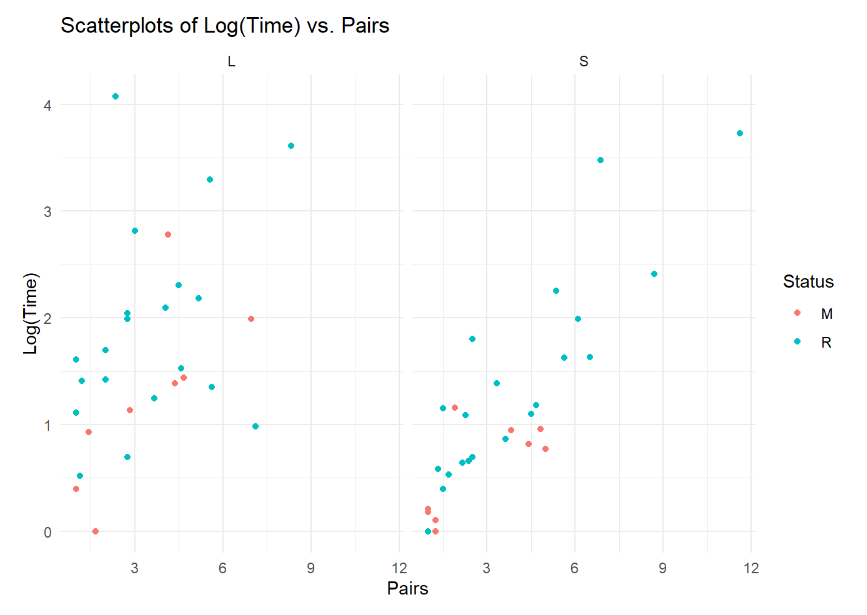
\includegraphics[scale=0.5]{graphs/graph5.png}
\end{center}

The relationship between log(Time) and Pairs does appear to be a positive linear relationship, thus indicating that a transformation of Pairs is not needed.

The relationship also appears to be more linear than with log-transformed Pairs, as shown below, where a slight curve pattern emerges.



\section{Exercise 6}

\subsection*{6.1}

\begin{center}
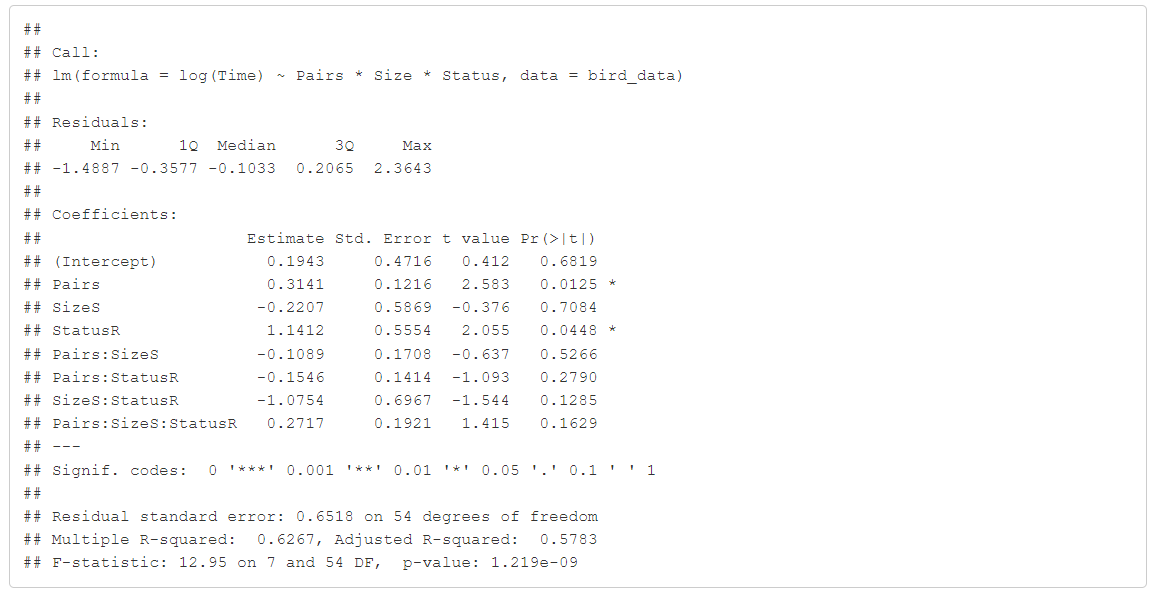
\includegraphics[scale=0.5]{tables/log-time.png}
\end{center}


After running this code, you will see the coefficients for each term in the model, including the interactions. To determine whether the slopes are equal for all combinations of “size” and “migratory status,” examine the coefficients for the interaction terms Pairs:Size, Pairs:Status, and Pairs:Size:Status. If the interaction terms are not statistically significant (i.e., their p-values are larger than a chosen significance level, typically 0.05), it suggests that the slopes are not significantly different between the four combinations of “size” and “migratory status.” \\

Pairs:SizeS: The coefficient is -0.1089 with a p-value of 0.5266, which is not statistically significant at a 0.05 significance level. \\

Pairs:StatusR: The coefficient is -0.1546 with a p-value of 0.2790, which is not statistically significant at a 0.05 significance level. \\

Pairs:SizeS:StatusR: The coefficient is 0.2717 with a p-value of 0.1629, which is not statistically significant at a 0.05 significance level. \\

Since none of the interaction terms are statistically significant, there is not enough evidence to conclude that the slopes for all four combinations of “size” and “migratory status” are different. This suggests that the relationship between “Pairs” and log(“Time”) may not be significantly different among the four groups based on “size” and “migratory status”. However, it is essential to note that a lack of statistical significance does not necessarily mean the slopes are equal; it indicates that there isn’t enough evidence to reject the null hypothesis that the slopes are equal.

\subsection*{6.2}
Nested models are a series of models where each model is a subset of the previous one. This approach helps in assessing the contribution of variables and their interactions to the overall model fit. To create nested models, start with the simplest model and gradually add variables and interaction terms to evaluate their contributions.


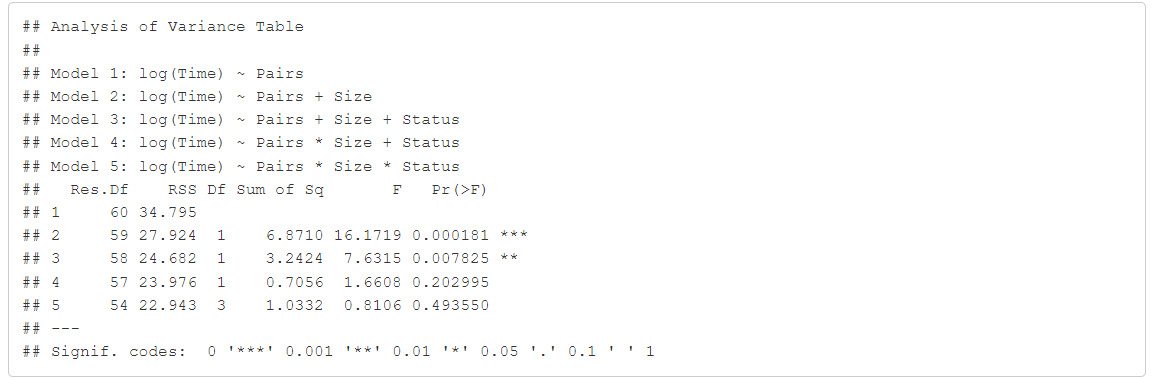
\includegraphics[scale=0.5]{tables/variance-table.png}


When we move from Model 1 to Model 2 (adding the Size variable), the p-value is 0.000181 (significant at the 0.05 level). This indicates that adding the Size variable significantly improves the model fit.

When we move from Model 2 to Model 3 (adding the Status variable), the p-value is 0.007825 (significant at the 0.05 level). This suggests that adding the Status variable significantly improves the model fit.

When we move from Model 3 to Model 4 (adding the Pairs * Size interaction term), the p-value is 0.202995 (not significant at the 0.05 level). This suggests that adding the Pairs * Size interaction term does not significantly improve the model fit.

When we move from Model 4 to Model 5 (adding the Pairs * Size * Status interaction term), the p-value is 0.493550 (not significant at the 0.05 level). This indicates that adding the Pairs * Size * Status interaction term does not significantly improve the model fit.

Based on the ANOVA results, it seems that Model 3 (Time ~ Pairs + Size + Status) is the most appropriate model for this dataset, as adding interaction terms does not significantly improve the model fit.

\section{Exercise 7}
Based on the findings from previous items, we can create a reduced model using just the Pairs, Size, and Status variables, without interaction terms.


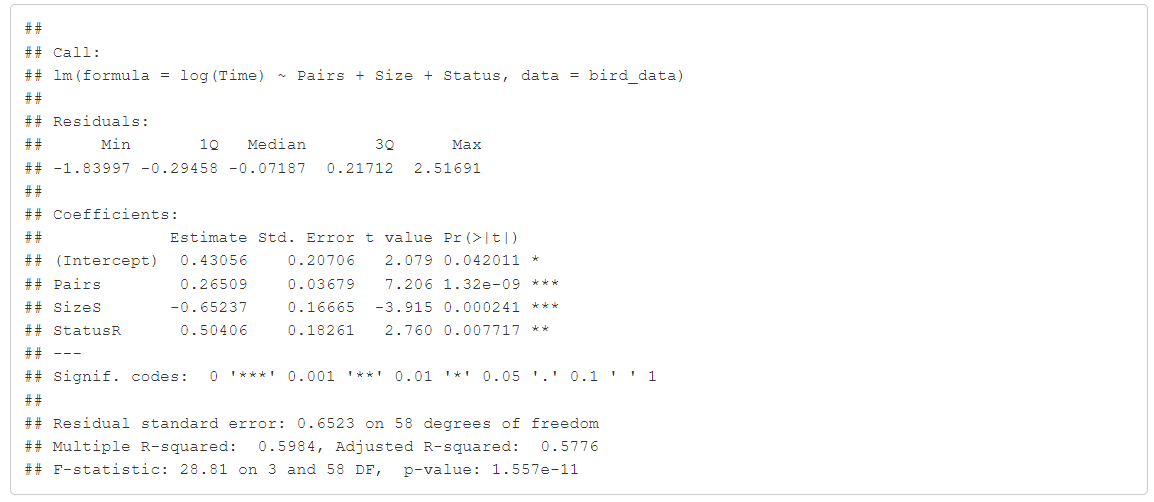
\includegraphics[scale=0.5]{tables/all-added.png}


\begin{center}
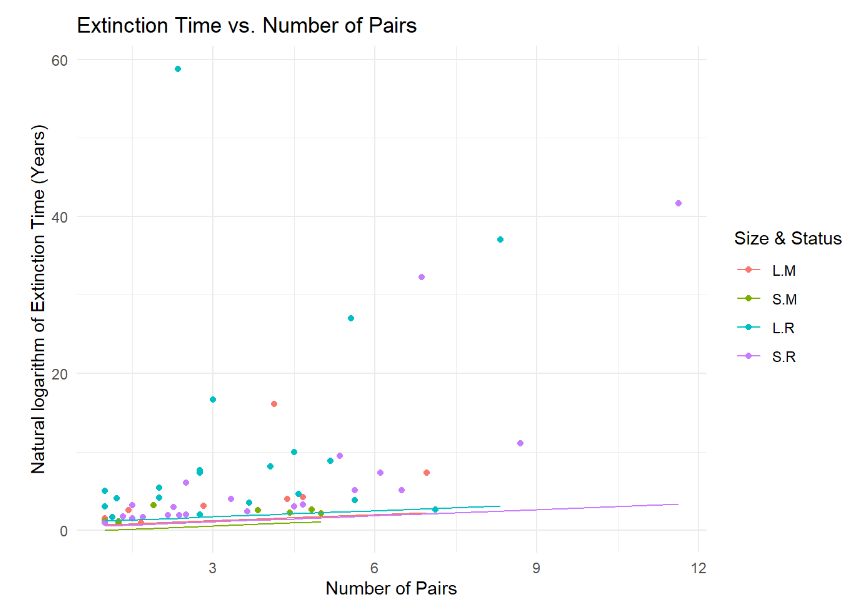
\includegraphics[scale=0.5]{graphs/graph7.png}
\end{center}

\section{Exercise 8}

After analyzing the data and accounting for the number of nesting pairs,
we can conclude that the number of nesting pairs has a significant
impact on the time it takes for a species to become extinct. Larger
numbers of nesting pairs tend to result in longer times before
extinction.

However, when considering the size and migratory status of species,
their individual effects on extinction time are less clear. We could not
establish a strong relationship between these factors and the time to
extinction, indicating that they may not be as influential as the number
of nesting pairs.

It is also worth noting that there were a few outliers with unusually
large extinction times compared to other species with similar
explanatory variable values. These outliers should be further
investigated to understand the underlying factors contributing to their
atypical extinction times.

Biggest outlier: \\
- Species: Raven \\
- Time: 58.82 \\
- Pairs: 2.35 \\
- Size: L \\ 
- Status: R \\

Based on the reduced model, the "theoretical" regression formula for the
logarithm of extinction time can be constructed using the coefficients
from the summary. The formula would look like this:

$$ln(Time) = 0.43056 + 0.26509 * Pairs - 0.65237 * SizeS + 0.50406 *
StatusR$$

Here,

ln(Time) represents the natural logarithm of the extinction time (note
that log() in R defaults to ln);

Pairs is the number of nesting pairs (as a continuous variable);

SizeS is a binary variable indicating the bird size, with 1 for
small-sized birds and 0 for large-sized birds;

StatusR is a binary variable indicating the migratory status, with 1 for
resident birds and 0 for migratory birds.

The coefficients in the formula represent the effects of each variable
on the logarithm of the extinction time while keeping the other
variables constant.

For example, an increase in the number of nesting pairs by one unit is
associated with an increase in the logarithm of extinction time by
0.26509 units, holding size and migratory status constant. Similarly,
small-sized birds have a 0.65237 units lower logarithm of extinction
time compared to large-sized birds, holding the number of nesting pairs
and migratory status constant.

This formula can be used as a conclusion to describe the relationship
between the extinction time and the variables of interest (number of
nesting pairs, size, and migratory status) based on the reduced model.




\end{document}